% =====================================================================
%  Bipolar (junction) Peltier cooling in PIN diodes:
%  why silicon is limited to millikelvin, why germanium does better,
%  and a research roadmap.
%  Compile:  pdflatex pin_peltier_si_vs_ge.tex   (run twice for references)
%  Packages: amsmath, siunitx, booktabs, pgfplots, tikz, tcolorbox, hyperref
% =====================================================================
\documentclass[11pt,a4paper]{article}

\usepackage[T1]{fontenc}
\usepackage[utf8]{inputenc}
\usepackage{lmodern}
\usepackage[margin=2.4cm]{geometry}
\usepackage{amsmath,amssymb,mathtools,bm}
\usepackage{siunitx}
\sisetup{separate-uncertainty=true, per-mode=symbol, range-phrase=--}
\usepackage{booktabs,tabularx,multirow,array}
\usepackage{graphicx}
\usepackage{xcolor}
\usepackage{tikz}
\usetikzlibrary{arrows.meta,decorations.pathreplacing,calc,positioning}
\usepackage{pgfplots}
\pgfplotsset{compat=1.17}
\usepackage{caption}
\captionsetup{font=small,labelfont=bf}
\usepackage{enumitem}
\setlist{nosep,leftmargin=*}
\usepackage[most]{tcolorbox}
\usepackage[colorlinks=true,linkcolor=blue!50!black,citecolor=green!40!black,urlcolor=blue!60!black]{hyperref}

% ---------------------------------------------------------------------
\newcommand{\kB}{k_{\mathrm{B}}}
\newcommand{\Eg}{E_{\mathrm{g}}}
\newcommand{\Ep}{E_{\mathrm{pair}}}
\newcommand{\Vj}{V_{\mathrm{j}}}
\newcommand{\VF}{V_{\mathrm{F}}}
\newcommand{\Da}{D_{\mathrm{a}}}
\newcommand{\Ca}{C_{\mathrm{a}}}
\newcommand{\nb}{n_{\mathrm{b}}}
\newcommand{\Pis}{\Pi_{\mathrm{side}}}
\newcommand{\Pit}{\Pi_{\mathrm{tot}}}
\newcommand{\Lh}{L_{\mathrm{h}}}
\newcommand{\Troom}{T_{\mathrm{room}}}
\newcommand{\nI}{n_{\mathrm{i}}}
\newcommand{\dd}{\mathrm{d}}

\newtcolorbox{insight}[1][]{colback=blue!3,colframe=blue!45!black,fonttitle=\bfseries,title={Physical insight#1},breakable}
\newtcolorbox{keyresult}[1][]{colback=green!4,colframe=green!40!black,fonttitle=\bfseries,title={Key result#1},breakable}
\newtcolorbox{caveat}[1][]{colback=orange!5,colframe=orange!60!black,fonttitle=\bfseries,title={Caveat#1},breakable}

\title{\textbf{Bipolar Junction Peltier Cooling in PIN Diodes}\\[4pt]
\large Why silicon is limited to millikelvin cooling, why germanium does better,\\
and a roadmap towards a high-impact publication}
\author{Thesis project report\\ \small (COMSOL~6.3 Semiconductor + Heat Transfer study, reference model and analysis)}
\date{\today}

\begin{document}
\maketitle

\begin{abstract}
\noindent A forward-biased PIN diode absorbs heat where electrons and holes are injected over the junction barriers and releases heat where they recombine. With an engineered recombination zone at the centre of the intrinsic region, the junctions become net heat sinks. A 51-run COMSOL campaign and a COMSOL-independent ambipolar reference model show that in silicon the effect is real but tiny: \SI{0.45}{\milli\kelvin} at \SI{0.7}{\volt} and an estimated \SIrange{20}{40}{\milli\kelvin} at the optimum bias near \SI{0.9}{\volt}. This report explains why from first principles. (i)~The heat absorbed per electron--hole pair is \emph{independent of the band gap} and depends only on the carrier density. (ii)~A ``lever-arm'' form of the heat equation shows that only recombination inside a small central fraction of each half of the device produces cooling. (iii)~The achievable temperature drop scales as $\nb\Da\Pis/k$, and Auger recombination caps the injected density. Together these give a closed-form ceiling $\Delta T_{\max}\propto(\Da\Pis)^{3/2}/(k\,W\sqrt{\Ep\Ca})$. Silicon's thermal conductivity ($k=\SI{148}{\watt\per\metre\per\kelvin}$) and modest ambipolar diffusivity ($\Da\approx\SI{18}{\centi\metre\squared\per\second}$) put it in the millikelvin range. Germanium combines a $3.6\times$ larger $\Da$ with a $2.5\times$ lower $k$. Its material figure of merit $\Da/k$ is therefore $8.9\times$ that of silicon, and the Auger-limited figure of merit is about $13$--$27\times$ larger. The reference model predicts \SIrange{0.15}{0.40}{\kelvin} for a germanium device with the same geometry, at only \SI{0.55}{\volt} and with a higher coefficient of performance. We close with five research directions grounded in the current literature, aimed at journals such as \emph{Physical Review Applied}, \emph{Nature Communications} and \emph{Nature Electronics}, and with a phase-by-phase COMSOL roadmap.
\end{abstract}

\tableofcontents
\newpage

% =====================================================================
\section{Introduction and what the simulations have shown so far}
% =====================================================================

\subsection{The device and the question}
The device is a one-dimensional silicon PIN diode: a \SI{2}{\micro\metre} $n^+$ layer and a \SI{2}{\micro\metre} $p^+$ layer (both \SI{1e19}{\per\centi\metre\cubed}) separated by a $W_i=\SI{1}{\milli\metre}$ intrinsic region with cross-section $A_c=\SI{1}{\milli\metre\squared}$. Under forward bias, electrons are injected from the $n^+$ side and holes from the $p^+$ side. They flood the intrinsic region (high injection, $n\approx p\gg\nI$) and recombine there. An optional recombination zone, a slab of short Shockley--Read--Hall (SRH) lifetime $\tau_{\mathrm{short}}$ and width $w_{\mathrm{rz}}$ at the centre, decides \emph{where} they recombine.

Two thermal configurations are used throughout:
\begin{itemize}
  \item \textbf{Config~A:} both ends held at $\Troom$, with a sink at the centre at $\Troom+\Delta T_{\mathrm{sink}}$. It gives the heat $Q_{\mathrm{room}}$ pumped out of the room and $\Delta T_{\max}$, the sink temperature rise at which $Q_{\mathrm{room}}=0$.
  \item \textbf{Config~B:} the centre held at $\Troom$ and the ends thermally insulated. For the symmetric bar, $\Troom-T_{\mathrm{end}}=\Delta T_{\max}$ of Config~A exactly.
\end{itemize}
The thermal problem is solved with one-way coupling: the semiconductor is solved at \SI{300}{\kelvin}, and its heat source $Q=\bm{J}\cdot\bm{E}+U(\Eg+3\kB T)$ plus the contact Peltier terms drives the heat equation.

\subsection{Summary of the results so far}
Table~\ref{tab:matrix} collects the key outputs.

\begin{table}[h]
\centering\footnotesize
\caption{Selected COMSOL results of the 51-run matrix (\SI{0.7}{\volt} unless stated) and the extended-bias reference model. $\Delta T$ = $\Troom-T_{\mathrm{end}}$ in Config~B, or $\Delta T_{\max}$ in Config~A.}
\label{tab:matrix}
\setlength{\tabcolsep}{4pt}
\begin{tabular}{llccc}
\toprule
Run & Change & $\Delta T$ (mK) & $Q_{\mathrm{room}}$ (mW) & Note\\
\midrule
V0 & uniform lifetime, \SI{1}{\milli\second} & $-0.152$ (heats) & $-0.090$ & room heated\\
V1 & zone \SI{100}{\micro\metre}/\SI{1}{\micro\second} & $0.447$ & $0.263$ & COP $=0.74$\\
V1 & same, best over $\VF\le\SI{0.8}{\volt}$ & $2.38$ & -- & at top of sweep\\
V3b & corrected heat source & $0.445$ & $0.262$ & $\eta_E=1.000$\\
V4 & mesh $\times2$ & $0.446$ & $0.263$ & converged (0.19\%)\\
V2b & FD + BGN + carrier--carrier scatt. & $0.386$ & $0.228$ & $-14\%$\\
V6 best & zone \SI{25}{\micro\metre}/\SI{1}{\micro\second} & $1.178$ & $0.695$ & optimum at \SI{0.7}{\volt}\\
V8b & Caughey--Thomas mobility, best & $2.56$ & -- & at \SI{0.8}{\volt}\\
\midrule
FINAL (ref.\ model) & zone \SI{25}{\micro\metre}/\SI{0.3}{\micro\second}, to \SI{1.5}{\volt} & $32.4$ & $19.2$ & peak \SI{0.92}{\volt}\\
\bottomrule
\end{tabular}
\end{table}

\noindent Three facts stand out:
\begin{enumerate}
  \item Uniform lifetime (V0) always heats the junction ends.
  \item An engineered central zone turns the device into a cooler, but even after optimising zone and bias the cooling stays in the tens of millikelvin. The COMSOL/reference ratio of 0.35--0.63 seen in the matrix suggests a COMSOL value of about \SIrange{10}{20}{\milli\kelvin} at the optimum.
  \item Modelling choices (mesh, heat-source form, mobility model) change the answer by less than \SI{15}{\percent}. The smallness is therefore physical, not numerical.
\end{enumerate}
Sections~\ref{sec:physics}--\ref{sec:silicon} explain why. Section~\ref{sec:ge} shows why germanium is better, Section~\ref{sec:novel} proposes research directions, and Section~\ref{sec:roadmap} gives the COMSOL roadmap.

% =====================================================================
\section{Physics of bipolar junction Peltier cooling}\label{sec:physics}
% =====================================================================

\subsection{A qualitative picture first}
Think of the junction barrier as a hill and the injected carriers as hikers.
\begin{itemize}
  \item Only the most energetic electrons of the $n^+$ reservoir can climb over the barrier into the intrinsic region. When they leave, they take more than the average energy with them, and the lattice at the junction has to supply it. This is \emph{evaporative cooling}, the same mechanism that cools a cup of coffee. The same happens to holes on the $p^+$ side.
  \item The injected electrons and holes then wander through the intrinsic region by \emph{ambipolar diffusion}. Electrons and holes move together because any separation creates an electric field that pulls them back together. Eventually they recombine, and recombination releases the full energy of the pair, about one band gap plus their thermal energy, as heat.
  \item The junction is therefore a \emph{cold source} and the recombination site a \emph{hot source}. Whether the ends end up colder than the centre depends on two questions: \emph{how far apart} the cold and hot sources are, and \emph{how easily heat flows back} from the hot source to the cold one.
\end{itemize}
These two questions, geometry of recombination and thermal back-flow, govern everything that follows.

\subsection{Energy book-keeping per electron--hole pair}
For non-degenerate carriers the mean kinetic energy is $\tfrac32\kB T$ per carrier. A recombining pair therefore releases
\begin{equation}
  \Ep = \Eg + 3\kB T \label{eq:Epair}
\end{equation}
into the lattice. This is exactly the recombination term $U(\Eg+3\kB T)$ of COMSOL's heat source~\cite{comsol,wachutka}.

The power supply delivers $q\VF$ per pair. In the intrinsic region the electron and hole quasi-Fermi levels are split by $q\Vj$, where $\Vj$ is the junction voltage: the part of $\VF$ that drops across the two junctions, as opposed to the resistive drop $V_i$ in the intrinsic region. Energy conservation per pair then requires the lattice on the \emph{cold sides} (junctions and contacts together) to supply
\begin{equation}
  \Pit \equiv \Ep - q\Vj , \qquad \Pis = \tfrac12\Pit \;\text{ per side.} \label{eq:Pitot}
\end{equation}
This is the bipolar Peltier coefficient of the device~\cite{pipe2002}. Applying more voltage injects more pairs, but each pair absorbs \emph{less} heat, because the barrier it climbs, $V_{\mathrm{bi}}-\Vj$, shrinks.

\subsection{The heat absorbed per pair does not depend on the band gap}
One might expect a wide-gap semiconductor to be a better cooler, since each pair carries $\Eg$ of energy. It is not, and the reason is instructive. To obtain a given carrier density $n$, a wide-gap material needs a correspondingly larger junction voltage. The gain in $\Ep$ is cancelled exactly by the larger $q\Vj$.

To show this, use the law of the junction in high injection. With $np=\nI^2\exp(q\Vj/\kB T)$ and $n=p$,
\begin{equation}
  n = \nI\, e^{q\Vj/2\kB T}
  \quad\Longrightarrow\quad
  q\Vj = 2\kB T\ln\frac{n}{\nI}. \label{eq:junction}
\end{equation}
Inserting the non-degenerate intrinsic density $\nI=\sqrt{N_cN_v}\,e^{-\Eg/2\kB T}$ into Eq.~\eqref{eq:Pitot}:
\begin{equation}
\boxed{\;
  \Pit = \Eg + 3\kB T - 2\kB T\ln\frac{n\,e^{\Eg/2\kB T}}{\sqrt{N_cN_v}}
       = 3\kB T + 2\kB T\,\ln\frac{\sqrt{N_c N_v}}{n}\; } \label{eq:Pi_universal}
\end{equation}

\begin{keyresult}[: band-gap independence]
The band gap cancels. At a given carrier density, the heat absorbed per pair depends only on temperature and on the effective densities of states. At $n=\SI{1e17}{\per\centi\metre\cubed}$ and \SI{300}{\kelvin}:
\begin{itemize}
  \item \textbf{Si} ($\sqrt{N_cN_v}=\SI{1.71e19}{\per\centi\metre\cubed}$): $\Pit=\SI{0.343}{\electronvolt}$.
  \item \textbf{Ge} ($\sqrt{N_cN_v}=\SI{7.9e18}{\per\centi\metre\cubed}$): $\Pit=\SI{0.304}{\electronvolt}$.
\end{itemize}
The heat \emph{per pair} is therefore not where materials differ. They differ in how many pairs can be pushed across per second (transport), how fast heat flows back (thermal conductivity), and how much voltage this costs (efficiency).
\end{keyresult}

\subsection{The lever-arm equation: where recombination happens matters}
\paragraph{Intuition.} Consider one half of the bar in Config~B. The end at $x=0$ is the cold junction, and the centre at $x=\Lh=W_i/2$ is held at $\Troom$. Heat released at a point $x$ must flow to the centre sink. On its way it raises the temperature of everything between $x$ and the centre, but \emph{not} the region beyond $x$ towards the end. Seen from the cold end, a heat source at $x$ therefore acts through a ``lever arm'' $(\Lh-x)$. Heat released near the end counts fully; heat released at the centre does not count at all.

\paragraph{Derivation.} In steady state, Fourier's law $q_x=-k\,\dd T/\dd x$ and energy conservation $\dd q_x/\dd x=H(x)$ hold, with $H$ the volumetric heat source. The cold end absorbs the Peltier flux $s$, so $q_x(0)=-s$, and $T(\Lh)=\Troom$. Integrating twice gives
\begin{equation}
  \boxed{\;\Delta T \equiv \Troom - T(0) = \frac1k\left[\, s\,\Lh - \int_0^{\Lh}(\Lh-x)\,H(x)\,\dd x \right]\;} \label{eq:lever}
\end{equation}
In the symmetric device, every pair injected through this end recombines in this half. The pair flux $\Gamma=J/q$ is therefore $\Gamma=\int_0^{\Lh}R(x)\,\dd x$, where $R$ is the recombination rate. The Peltier flux is $s=\Pis\Gamma$, and the heat source is $H=\Ep R+\bm J\cdot\bm E$. Substituting,
\begin{equation}
  \Delta T = \frac1k\int_0^{\Lh} R(x)\Big[\underbrace{\Pis\Lh}_{\text{cooling credit}} - \underbrace{\Ep(\Lh-x)}_{\text{heating debit}}\Big]\dd x \;-\; \Delta T_{\mathrm{J}}, \label{eq:lever2}
\end{equation}
where $\Delta T_{\mathrm J}$ is the Joule contribution. Each recombination event earns a fixed cooling credit and pays a heating debit that grows with its distance from the centre. It produces net cooling only if it happens beyond the break-even point
\begin{equation}
  x^\ast = \Lh\left(1-\frac{\Pis}{\Ep}\right). \label{eq:xstar}
\end{equation}

\begin{insight}[: why uniform lifetime can never cool]
With $\Pis=\tfrac12(\Ep-q\Vj)$, we have $\Pis/\Ep<\tfrac12$ always. For silicon at the optimum ($\Vj\approx\SI{0.85}{\volt}$), $\Pis/\Ep\approx0.14$, so only recombination in the \textbf{innermost \SI{14}{\percent}} of each half cools. If recombination were uniform, the average lever arm would be $\Lh/2$, and the bracket in Eq.~\eqref{eq:lever2} would average to $\Lh(\Pis-\Ep/2)<0$. \emph{Uniform recombination always heats the ends}. In a real uniform-lifetime diode the carrier density, and with it the recombination, is highest near the junctions, which makes it worse. This is exactly the V0 result, and it is why the recombination zone is indispensable.
\end{insight}

\begin{figure}[h]
\centering
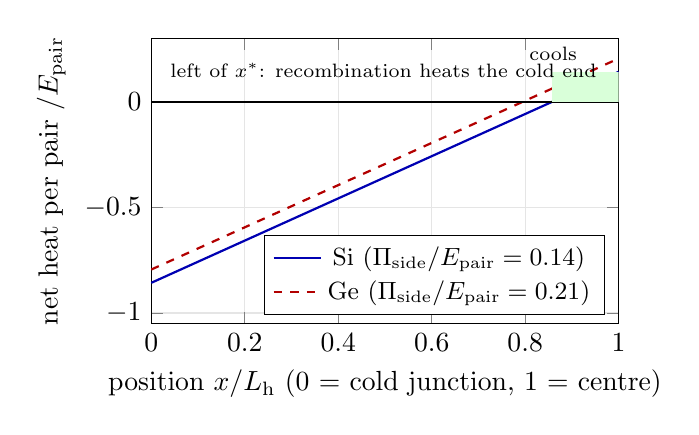
\begin{tikzpicture}
\begin{axis}[width=0.62\textwidth,height=5.2cm,xmin=0,xmax=1,ymin=-1.05,ymax=0.3,
  xlabel={position $x/\Lh$ (0 = cold junction, 1 = centre)},ylabel={net heat per pair $/\Ep$},
  grid=major,grid style={gray!20},legend pos=south east,legend style={font=\small}]
\addplot[domain=0:1,thick,blue!70!black]{0.143-(1-x)};
\addlegendentry{Si ($\Pis/\Ep=0.14$)}
\addplot[domain=0:1,thick,red!70!black,dashed]{0.206-(1-x)};
\addlegendentry{Ge ($\Pis/\Ep=0.21$)}
\addplot[black,thin] coordinates {(0,0) (1,0)};
\fill[green!15] (axis cs:0.857,0) rectangle (axis cs:1,0.143);
\node[font=\scriptsize,anchor=south] at (axis cs:0.86,0.15) {cools};
\node[font=\scriptsize,anchor=west] at (axis cs:0.02,0.15) {left of $x^\ast$: recombination heats the cold end};
\end{axis}
\end{tikzpicture}
\caption{Lever-arm weight $[\Pis\Lh-\Ep(\Lh-x)]/(\Ep\Lh)$ of Eq.~\eqref{eq:lever2}, evaluated at each material's optimum bias ($n\approx\SI{1e17}{\per\centi\metre\cubed}$). Recombination contributes net cooling only to the right of $x^\ast$.}
\label{fig:lever}
\end{figure}

\subsection{Diffusion-limited pumping: the scaling $\Delta T\simeq \nb\Da\Pis/k$}
\paragraph{Intuition.} Suppose the zone were a perfect sink at the centre. All the cooling credit then comes from how many pairs reach the centre per second. In high injection, pairs move by ambipolar diffusion down a concentration gradient, so the pair flux is set by the boundary density $\nb$ and the diffusivity. Back-conduction of heat is set by $k$.

\paragraph{Equations.} For a perfect central sink the profile is linear, $n(x)=\nb(1-x/\Lh)$, and
\begin{equation}
  \Gamma = \frac{\Da\nb}{\Lh}, \qquad
  \Da=\frac{2D_nD_p}{D_n+D_p}=\frac{\kB T}{q}\,\frac{2\mu_n\mu_p}{\mu_n+\mu_p}. \label{eq:flux}
\end{equation}
Putting all recombination at $x=\Lh$ in Eq.~\eqref{eq:lever2} gives
\begin{equation}
  \boxed{\;\Delta T_{\mathrm{ideal}} = \frac{\Lh\,\Gamma\,\Pis}{k} = \frac{\nb\,\Da\,\Pis}{k}\;} \label{eq:ideal}
\end{equation}
The device length cancels: a shorter device pumps more heat ($\Gamma\propto1/\Lh$) but also conducts more heat back, by the same factor. The V5 runs at \SI{0.7}{\volt} confirm this length independence.

A zone of finite strength, with sink velocity $S\approx w_{\mathrm{rz}}/(2\tau_{\mathrm{short}})$ per side, acts as a series ``resistance'' to the pair flux:
\begin{equation}
  \Gamma=\frac{\nb}{\Lh/\Da+1/S}\quad\Longrightarrow\quad
  \Delta T = \frac{\nb\Da\Pis}{k}\;\frac{1}{1+\Da/(S\Lh)} . \label{eq:finiteS}
\end{equation}
Cooling therefore needs $S\gg\Da/\Lh$, which is \SI{360}{\centi\metre\per\second} for silicon. This is consistent with the V6 optimum, $S\approx\SIrange{500}{2500}{\centi\metre\per\second}$. If the zone is too strong, it drains the carriers, the intrinsic region becomes resistive, and at fixed $\VF$ the junction voltage, and with it $\nb$, falls.

\subsection{The Auger ceiling}
\paragraph{Intuition.} Raising the bias raises $\nb$ exponentially. Why, then, is there an optimum? Auger recombination, in which three carriers are involved, grows as $n^3$. It happens wherever the density is high, which is right next to the cold junction, where the lever arm is longest. Beyond a certain density these ``wrong-place'' recombination events dominate.

\paragraph{Equations.} Take the Auger rate $R_A=\Ca n^3$ (ambipolar coefficient $\Ca$) on the linear profile and insert it as a heating debit into Eq.~\eqref{eq:lever}:
\begin{equation}
  \Delta T_A = \frac{\Ep\Ca}{k}\int_0^{\Lh}\nb^3\Big(1-\frac{x}{\Lh}\Big)^3(\Lh-x)\,\dd x = \frac{\Ep\Ca\nb^3\Lh^2}{5k}. \label{eq:auger}
\end{equation}
The net temperature drop as a function of the injected density is then
\begin{equation}
  \Delta T(\nb)\simeq\frac1k\left[\Pis\Da\nb-\frac{\Ep\Ca\Lh^2}{5}\nb^3\right]. \label{eq:dTn}
\end{equation}
It is maximal at
\begin{equation}
  n_{\mathrm{opt}} = \frac{1}{\Lh}\sqrt{\frac{5\,\Pis\Da}{3\,\Ep\Ca}}, \qquad
  \boxed{\;\Delta T_{\max}^{\mathrm{Auger}} = \frac{2}{3}\frac{n_{\mathrm{opt}}\Da\Pis}{k}
  = \frac{2}{3\,k\,\Lh}\,(\Pis\Da)^{3/2}\sqrt{\frac{5}{3\,\Ep\Ca}}\;} \label{eq:dTmax}
\end{equation}
Two consequences follow. First, the material enters through the combination
\begin{equation}
  \mathcal F \equiv \frac{(\Da\Pis)^{3/2}}{k\sqrt{\Ep\Ca}},  \label{eq:F}
\end{equation}
which we call the \emph{Auger-limited figure of merit}. Second, at the Auger limit the length \emph{does} matter: $\Delta T_{\max}\propto1/W_i$, because a shorter device needs less density for the same flux. This is not seen at \SI{0.7}{\volt}, where the device is far from the Auger limit.

\subsection{Joule heating is a minor term}
With $\sigma(x)=q(\mu_n+\mu_p)n(x)$ on the linear profile, the Joule contribution to Eq.~\eqref{eq:lever} is
\begin{equation}
  \Delta T_{\mathrm J}=\frac1k\int_0^{\Lh}\frac{J^2}{\sigma(x)}(\Lh-x)\,\dd x=\frac{J^2\Lh^2}{q(\mu_n+\mu_p)\nb k}.
\end{equation}
Relative to Eq.~\eqref{eq:ideal}, using Eq.~\eqref{eq:flux},
\begin{equation}
  \frac{\Delta T_{\mathrm J}}{\Delta T_{\mathrm{ideal}}} = \frac{\kB T}{\Pis}\,\frac{2\mu_n\mu_p}{(\mu_n+\mu_p)^2}\approx
  \begin{cases}0.06 & \text{Si}\\ 0.08 & \text{Ge}\end{cases} \label{eq:joule}
\end{equation}
Joule heating in the intrinsic region costs only a few per cent. The limits are the lever arm, the Auger rate, and the ratio $\Da/k$. Joule heating takes over only beyond the optimum, when $\Vj\to V_{\mathrm{bi}}$ and every extra volt drops resistively; this is the heating seen above about \SI{1}{\volt} in the extended sweep.

% =====================================================================
\section{Why silicon is limited to millikelvin cooling}\label{sec:silicon}
% =====================================================================

\subsection{Numbers}
For silicon the parameters are\\ $\Da=\SI{18.3}{\centi\metre\squared\per\second}$ ($\mu_n=1414$, $\mu_p=\SI{471}{\centi\metre\squared\per\volt\per\second}$), $k=\SI{148}{\watt\per\metre\per\kelvin}$~\cite{glassbrenner}, $\Ep=\SI{1.198}{\electronvolt}$, $\Pis\approx\SI{0.172}{\electronvolt}$ at \SI{1e17}{\per\centi\metre\cubed}, and the Dziewior--Schmid $\Ca=C_n+C_p=\SI{3.8e-31}{\centi\metre\tothe{6}\per\second}$~\cite{dziewior}. Equation~\eqref{eq:dTmax} then gives
\begin{equation}
 n_{\mathrm{opt}}\approx\SI{6.8e16}{\per\centi\metre\cubed},\qquad \Delta T_{\max}^{\mathrm{Auger}}\approx\SI{15}{\milli\kelvin}.
\end{equation}
The ambipolar Auger coefficient measured at high injection, $\Ca=\SI{1.66e-30}{\centi\metre\tothe{6}\per\second}$~\cite{sinton}, gives $\SI{7}{\milli\kelvin}$. The full reference model, which also credits the Peltier heat of Auger pairs that cross the junction, gives \SIrange{32}{37}{\milli\kelvin} (Dziewior--Schmid) or \SI{21}{\milli\kelvin} (high-injection Auger). The analytic ceiling is within a factor of about 2.4 of the full model, and both say ``tens of millikelvin at best''.

\subsection{The reason in one sentence}
\begin{keyresult}[: why silicon gives millikelvin]
Silicon conducts heat about a hundred times too well for the rate at which ambipolar diffusion can deliver pairs to the recombination zone, and Auger recombination stops us from compensating with a higher carrier density. With $\Da/k=\SI{1.2e-5}{\metre\cubed\kelvin\per\joule}$, even $\nb=\SI{1e17}{\per\centi\metre\cubed}$ and $\Pis=\SI{0.17}{\electronvolt}$ give only $\nb\Da\Pis/k\approx\SI{34}{\milli\kelvin}$ in the ideal limit.
\end{keyresult}

\subsection{An equivalent view: the device as a poor thermoelectric}
A thermoelectric leg reaches $\Delta T_{\max}=\tfrac12 ZT_c^2$ with $Z=S^2\sigma/k$~\cite{goldsmid}. Define for the PIN an effective Seebeck coefficient $S_{\mathrm{eff}}=\Pis/(qT)$ and a conductivity $\sigma=q\nb(\mu_n+\mu_p)$. At $\nb=\SI{1e17}{\per\centi\metre\cubed}$:
\begin{center}\small
\begin{tabular}{lcccc}
\toprule
 & $S_{\mathrm{eff}}$ (\si{\micro\volt\per\kelvin}) & $\sigma$ (\si{\siemens\per\metre}) & $ZT$ & $\tfrac12ZT^2$ (K) \\
\midrule
Si PIN & 573 & 3.0e3 & 0.002 & 0.30\\
Ge PIN & 507 & 9.3e3 & 0.012 & 1.8\\
Bi$_2$Te$_3$ (for scale) & $\sim$200 & $\sim$1e5 & $\sim$1 & $\sim$70\\
\bottomrule
\end{tabular}
\end{center}
The Seebeck coefficient of the bipolar junction is \emph{large}, about $3\times$ that of Bi$_2$Te$_3$. What is fatal is $\sigma/k$, which is about 1000 times worse. The real device stays about $10\times$ below even this optimistic bound, because transport is diffusive and recombining, not ohmic. Silicon's $ZT\approx0.002$ is the thermoelectric way of saying ``millikelvin''.

\subsection{Can engineering rescue silicon?}
\begin{itemize}
  \item \textbf{Shorter devices:} $\Delta T_{\max}^{\mathrm{Auger}}\propto1/W_i$, but the current density scales as $\Gamma\propto n_{\mathrm{opt}}/\Lh\propto1/W_i^2$. A $20\times$ gain ($W_i=\SI{50}{\micro\metre}$) would require current densities of order \SI{e4}{\ampere\per\centi\metre\squared} and kW\,cm$^{-2}$ heat fluxes. This is not practical.
  \item \textbf{Higher bias:} beyond the optimum ($\approx\SI{0.92}{\volt}$) Auger heat and the vanishing barrier ($\Vj\to V_{\mathrm{bi}}$) turn cooling into heating (Fig.~\ref{fig:dT}).
  \item \textbf{Lower $k$ by nanostructuring} (holey Si $\sim\SI{2}{\watt\per\metre\per\kelvin}$~\cite{tang2010}, rough nanowires~\cite{hochbaum}): $\Delta T\propto1/k$, so this is the only strong lever. The surfaces it introduces, however, destroy the lifetimes and mobilities on which $\Da$ and the zone design rely, unless they are passivated to $S\lesssim\SI{10}{\centi\metre\per\second}$.
\end{itemize}

% =====================================================================
\section{Why germanium gives better results}\label{sec:ge}
% =====================================================================

\subsection{Intuition}
Equation~\eqref{eq:Pi_universal} showed that the band gap is irrelevant for the heat per pair, and Eqs.~\eqref{eq:ideal} and~\eqref{eq:dTmax} showed what matters: carriers that diffuse fast ($\Da$), a lattice that conducts heat poorly ($k$), and weak Auger recombination ($\Ca$). Germanium is a better conductor of \emph{carriers}, with both electron and hole mobilities 2.8--4 times higher than in silicon, and a worse conductor of \emph{heat}, because of its heavier atoms and softer lattice. Its narrow gap gives an additional, independent bonus: by Eq.~\eqref{eq:junction}, the same carrier density is reached at roughly half the voltage, so each pair costs half the electrical energy.

\subsection{Material parameters}
\begin{table}[h]
\centering\small
\caption{Parameters at \SI{300}{\kelvin} used in this report.}
\label{tab:params}
\setlength{\tabcolsep}{4pt}
\begin{tabular}{lccl}
\toprule
Quantity & Si & Ge & Source\\
\midrule
$\Eg$ (eV) & 1.12 & 0.66 & \cite{sze}\\
$N_c$, $N_v$ (\si{\per\centi\metre\cubed}) & 2.8e19, 1.04e19 & 1.04e19, 6.0e18 & COMSOL library~\cite{comsol}, \cite{sze}\\
$\nI$ (\si{\per\centi\metre\cubed}) & 9.65e9 (ref.\ model) & 2.0e13 & \cite{sze}\\
$\mu_n$, $\mu_p$ (\si{\centi\metre\squared\per\volt\per\second}) & 1414, 471 & 3900, 1900 & \cite{caughey,sze}\\
$\Da$ (\si{\centi\metre\squared\per\second}) & 18.3 & 66.0 & Eq.~\eqref{eq:flux}\\
$k$ (\si{\watt\per\metre\per\kelvin}) & 148 & 60 & \cite{glassbrenner}\\
$\Ca$ (\si{\centi\metre\tothe{6}\per\second}) & 3.8e-31 / 1.66e-30 & 7e-31 & \cite{dziewior,sinton}, \cite{garin2026}\\
$\Ep=\Eg+3\kB T$ (eV) & 1.198 & 0.738 & Eq.~\eqref{eq:Epair}\\
$\Pit$ at \SI{1e17}{\per\centi\metre\cubed} (eV) & 0.343 & 0.304 & Eq.~\eqref{eq:Pi_universal}\\
$\Vj$ for \SI{1e17}{\per\centi\metre\cubed} (V) & 0.85 & 0.44 & Eq.~\eqref{eq:junction}\\
\midrule
$M=\Da/k$ (\si{\metre\cubed\kelvin\per\joule}) & 1.24e-5 & 1.10e-4 & ratio $\mathbf{8.9}$\\
$\mathcal F$, Eq.~\eqref{eq:F} (relative) & 1 & $\mathbf{13}$ / $\mathbf{27}$ & vs.\ Si $\Ca$ (DS / high inj.)\\
\bottomrule
\end{tabular}
\end{table}

\subsection{Mathematical comparison}
\paragraph{Diffusion-limited regime.} At equal $\nb$, Eq.~\eqref{eq:ideal} gives
\begin{equation}
  \frac{\Delta T_{\mathrm{Ge}}}{\Delta T_{\mathrm{Si}}}
  =\frac{(\Da/k)_{\mathrm{Ge}}}{(\Da/k)_{\mathrm{Si}}}\cdot\frac{\Pis^{\mathrm{Ge}}}{\Pis^{\mathrm{Si}}}
  = 8.9\times0.88\approx 7.8 .
\end{equation}

\paragraph{Auger-limited optimum.} From Eq.~\eqref{eq:dTmax},
\begin{equation}
  \frac{\Delta T^{\mathrm{Ge}}_{\max}}{\Delta T^{\mathrm{Si}}_{\max}}
  =\left[\frac{(\Da\Pis)_{\mathrm{Ge}}}{(\Da\Pis)_{\mathrm{Si}}}\right]^{3/2}
   \frac{k_{\mathrm{Si}}}{k_{\mathrm{Ge}}}
   \sqrt{\frac{(\Ep\Ca)_{\mathrm{Si}}}{(\Ep\Ca)_{\mathrm{Ge}}}}
  = 3.2^{3/2}\times2.47\times\begin{cases}0.94\\ 1.96\end{cases}
\end{equation}
which is about $13$ when silicon is given the Dziewior--Schmid Auger coefficient, and about $27$ when it is given the high-injection value.
In absolute terms the formula gives $n_{\mathrm{opt}}\approx\SI{1.1e17}{\per\centi\metre\cubed}$ and $\Delta T^{\mathrm{Auger}}_{\max}\approx\SI{0.20}{\kelvin}$ for germanium.

\paragraph{Voltage and efficiency.} Per pair, the electrical cost is $q\VF\gtrsim q\Vj$ and the cold-side gain is $\Pit$. The ideal per-pair coefficient of performance, ignoring back-conduction, is
\begin{equation}
  \mathrm{COP}_0\simeq\frac{\Pit}{q\VF}\approx\frac{\Ep-q\Vj}{q\Vj}
  \approx\begin{cases}0.40 & \text{Si}\\ 0.68 & \text{Ge}\end{cases}\qquad(n=\SI{1e17}{\per\centi\metre\cubed}).
\end{equation}
Germanium therefore cools with about 1.7 times less electrical work per unit of heat.

\subsection{Reference-model results}
The COMSOL-independent reference model, which solves the ambipolar boundary-value problem with SRH, Auger and the exact heat integration, was run for both materials with identical geometry ($W_i=\SI{1}{\milli\metre}$, \SI{25}{\micro\metre} zone, $\tau_{\mathrm{long}}=\SI{1}{\milli\second}$). Germanium was given the parameters of Table~\ref{tab:params}.

\begin{table}[h]
\centering\small
\caption{Peak cooling over bias (Config~B, reference model).}
\label{tab:ref}
\begin{tabular}{lccccc}
\toprule
Case & $\tau_{\mathrm{short}}$ & peak $\Delta T$ & at $\VF$ & COP & $P_{\mathrm{el}}$\\
\midrule
Si, $\Ca$ (DS) & \SI{0.3}{\micro\second} & \SI{32}{\milli\kelvin} & \SI{0.92}{\volt} & 0.20 & \SI{96}{\milli\watt}\\
Si, $\Ca$ (DS) & \SI{0.1}{\micro\second} & \SI{37}{\milli\kelvin} & \SI{0.97}{\volt} & 0.20 & \SI{110}{\milli\watt}\\
Si, $\Ca$ (high injection) & \SI{0.1}{\micro\second} & \SI{22}{\milli\kelvin} & \SI{0.94}{\volt} & 0.23 & \SI{55}{\milli\watt}\\
\textbf{Ge} & \SI{0.1}{\micro\second} & \textbf{\SI{348}{\milli\kelvin}} & \SI{0.55}{\volt} & 0.28 & \SI{295}{\milli\watt}\\
\textbf{Ge} & \SI{0.03}{\micro\second} & \textbf{\SI{397}{\milli\kelvin}} & \SI{0.61}{\volt} & 0.26 & \SI{365}{\milli\watt}\\
Ge, mobilities $\times0.5$ (carrier--carrier) & \SI{0.1}{\micro\second} & \SI{149}{\milli\kelvin} & \SI{0.57}{\volt} & 0.29 & \SI{125}{\milli\watt}\\
Ge, $W_i=\SI{0.5}{\milli\metre}$ & \SI{0.01}{\micro\second} & \SI{600}{\milli\kelvin} & \SI{0.69}{\volt} & 0.20 & \SI{1.48}{\watt}\\
\bottomrule
\end{tabular}
\end{table}

\begin{figure}[h]
\centering
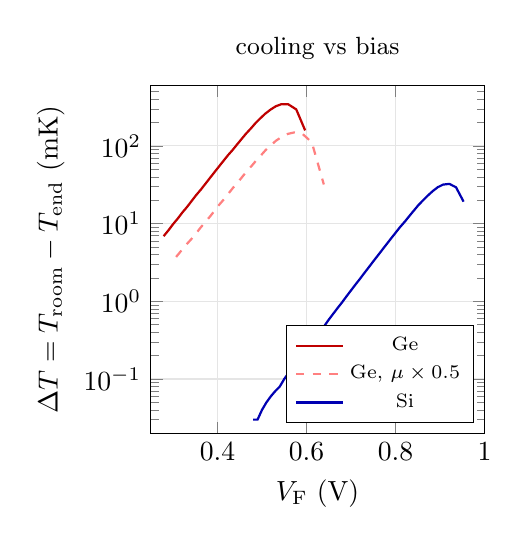
\begin{tikzpicture}
\begin{semilogyaxis}[width=0.48\textwidth,height=6cm,xmin=0.25,xmax=1.0,ymin=0.02,ymax=600,
  xlabel={$\VF$ (V)},ylabel={$\Delta T=\Troom-T_{\mathrm{end}}$ (mK)},
  grid=major,grid style={gray!20},legend pos=south east,legend style={font=\scriptsize},title={\small cooling vs bias}]
\addplot[thick,red!75!black] coordinates {(0.279,6.890) (0.290,8.220) (0.300,9.800) (0.311,11.660) (0.321,13.870) (0.332,16.480) (0.342,19.570) (0.352,23.220) (0.363,27.530) (0.373,32.610) (0.383,38.610) (0.393,45.670) (0.403,53.970) (0.413,63.720) (0.423,75.160) (0.434,88.550) (0.444,104.180) (0.454,122.360) (0.464,143.400) (0.475,167.550) (0.485,194.970) (0.496,225.530) (0.507,258.570) (0.519,292.400) (0.531,323.440) (0.544,344.690) (0.559,343.040) (0.577,294.810) (0.597,158.240)};
\addlegendentry{Ge}
\addplot[thick,red!50,dashed] coordinates {(0.307,3.720) (0.318,4.440) (0.329,5.290) (0.341,6.290) (0.352,7.480) (0.362,8.880) (0.373,10.530) (0.384,12.490) (0.394,14.800) (0.404,17.520) (0.415,20.720) (0.425,24.490) (0.435,28.910) (0.446,34.100) (0.456,40.160) (0.466,47.240) (0.477,55.450) (0.487,64.940) (0.498,75.800) (0.508,88.070) (0.520,101.620) (0.531,116.040) (0.544,130.390) (0.558,142.680) (0.573,149.130) (0.591,142.760) (0.612,111.010) (0.639,31.860)};
\addlegendentry{Ge, $\mu\times0.5$}
\addplot[thick,blue!70!black] coordinates {(0.480,0.030) (0.490,0.030) (0.500,0.040) (0.510,0.050) (0.520,0.060) (0.530,0.070) (0.540,0.080) (0.550,0.100) (0.560,0.120) (0.570,0.140) (0.580,0.170) (0.590,0.200) (0.600,0.240) (0.610,0.280) (0.620,0.340) (0.630,0.400) (0.640,0.480) (0.650,0.580) (0.660,0.690) (0.670,0.820) (0.680,0.970) (0.690,1.160) (0.700,1.380) (0.710,1.640) (0.720,1.940) (0.730,2.310) (0.740,2.740) (0.750,3.260) (0.760,3.860) (0.770,4.580) (0.780,5.430) (0.790,6.430) (0.800,7.600) (0.810,8.980) (0.821,10.600) (0.831,12.480) (0.841,14.650) (0.851,17.150) (0.862,19.950) (0.873,23.040) (0.884,26.270) (0.895,29.370) (0.907,31.770) (0.921,32.420) (0.936,29.360) (0.953,19.170)};
\addlegendentry{Si}
\end{semilogyaxis}
\end{tikzpicture}\hfill
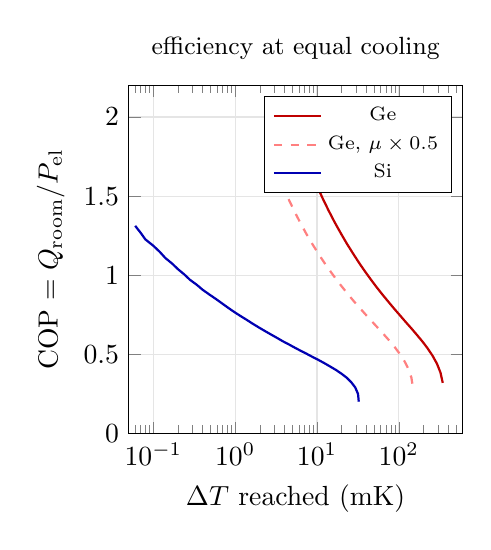
\begin{tikzpicture}
\begin{semilogxaxis}[width=0.48\textwidth,height=6cm,xmin=0.05,xmax=600,ymin=0,ymax=2.2,
  xlabel={$\Delta T$ reached (mK)},ylabel={COP $=Q_{\mathrm{room}}/P_{\mathrm{el}}$},
  grid=major,grid style={gray!20},legend pos=north east,legend style={font=\scriptsize},title={\small efficiency at equal cooling}]
\addplot[thick,red!75!black] coordinates {(6.890,1.769) (8.220,1.668) (9.800,1.575) (11.660,1.489) (13.870,1.409) (16.480,1.334) (19.570,1.265) (23.220,1.199) (27.530,1.138) (32.610,1.079) (38.610,1.024) (45.670,0.972) (53.970,0.922) (63.720,0.875) (75.160,0.830) (88.550,0.786) (104.180,0.744) (122.360,0.702) (143.400,0.662) (167.550,0.621) (194.970,0.580) (225.530,0.537) (258.570,0.491) (292.400,0.441) (323.440,0.384) (344.690,0.319) (344.690,0.319)};
\addlegendentry{Ge}
\addplot[thick,red!50,dashed] coordinates {(3.720,1.577) (4.440,1.487) (5.290,1.405) (6.290,1.329) (7.480,1.258) (8.880,1.193) (10.530,1.132) (12.490,1.074) (14.800,1.020) (17.520,0.968) (20.720,0.920) (24.490,0.873) (28.910,0.829) (34.100,0.787) (40.160,0.746) (47.240,0.706) (55.450,0.667) (64.940,0.628) (75.800,0.589) (88.070,0.549) (101.620,0.506) (116.040,0.461) (130.390,0.410) (142.680,0.352) (149.130,0.286) (149.130,0.286)};
\addlegendentry{Ge, $\mu\times0.5$}
\addplot[thick,blue!70!black] coordinates {(0.060,1.312) (0.070,1.268) (0.080,1.226) (0.100,1.186) (0.120,1.147) (0.140,1.109) (0.170,1.073) (0.200,1.038) (0.240,1.004) (0.280,0.971) (0.340,0.939) (0.400,0.908) (0.480,0.879) (0.580,0.850) (0.690,0.822) (0.820,0.794) (0.970,0.768) (1.160,0.742) (1.380,0.718) (1.640,0.693) (1.940,0.670) (2.310,0.647) (2.740,0.625) (3.260,0.603) (3.860,0.581) (4.580,0.561) (5.430,0.540) (6.430,0.520) (7.600,0.501) (8.980,0.481) (10.600,0.462) (12.480,0.442) (14.650,0.421) (17.150,0.400) (19.950,0.377) (23.040,0.352) (26.270,0.323) (29.370,0.290) (31.770,0.249) (32.420,0.200) (32.420,0.200)};
\addlegendentry{Si}
\end{semilogxaxis}
\end{tikzpicture}
\caption{Reference-model comparison at identical geometry. Si: \SI{25}{\micro\metre}/\SI{0.3}{\micro\second} zone (the FINAL design). Ge: \SI{25}{\micro\metre}/\SI{0.1}{\micro\second}. Left: germanium cools about $10\times$ more, at about \SI{0.4}{\volt} lower bias. Right: COP against the cooling reached (rising branch up to each peak); at any given cooling level germanium needs less electrical power. Only positive $\Delta T$ is shown on the log scale; both devices heat beyond their peak.}
\label{fig:dT}
\end{figure}

\begin{keyresult}[: germanium]
At identical geometry and an optimised zone, germanium cools about $10\times$ more than silicon (\SIrange{0.35}{0.40}{\kelvin} against \SIrange{0.03}{0.04}{\kelvin} in the reference model). It does so at about \SI{0.55}{\volt} instead of \SI{0.92}{\volt}, with a higher COP, and in agreement with the analytic ratio of 8--13. Including the strong carrier--carrier scattering recently measured in Ge at high injection~\cite{garin2026} (about $\times0.5$ on the mobilities) gives \SI{0.15}{\kelvin}. The realistic expectation, after COMSOL's typical factor of 0.4--0.6 with respect to the reference model, is therefore \textbf{about 0.1--0.2\,K for Ge, against 0.01--0.02\,K for Si}: one order of magnitude, but still sub-kelvin.
\end{keyresult}

\subsection{What could go wrong with germanium}
\begin{caveat}
\begin{enumerate}
  \item \textbf{Carrier--carrier scattering.} The sum $\mu_n+\mu_p$ falls roughly as $8\times10^{20}/\Delta n$\,\si{\centi\metre\squared\per\volt\per\second} at high injection~\cite{garin2026}, which bites exactly near $n_{\mathrm{opt}}$. It must be modelled (Fletcher model~\cite{fletcher} or a user-defined mobility).
  \item \textbf{Lifetime.} The bulk lifetime must exceed the transit time $\Lh^2/\Da\approx\SI{40}{\micro\second}$ by a wide margin. Bulk high-purity Ge can provide this; Ge-on-Si epitaxy, with its threading dislocations, cannot.
  \item \textbf{Contacts.} With $N_v=\SI{6e18}{\per\centi\metre\cubed}$, a $p^+$ layer at \SI{1e19}{\per\centi\metre\cubed} is degenerate. Fermi--Dirac statistics, or a lower doping (about \SI{3e18}{\per\centi\metre\cubed}), and recomputed contact Peltier terms are needed. Metal/$n$-Ge contacts suffer from strong Fermi-level pinning~\cite{dimoulas}.
  \item \textbf{Thermal feedback.} $P_{\mathrm{el}}\approx\SI{0.3}{\watt\per\milli\metre\squared}$ and $\Delta T\sim\SI{0.3}{\kelvin}$ approach the limit of one-way coupling. Since $\dd\ln\nI/\dd T\approx\SI{4.8}{\percent\per\kelvin}$, two-way electro-thermal coupling is required.
  \item \textbf{Plausibility threshold.} The project's automatic check flags cooling of \SI{0.1}{\kelvin} or more as a bug; that threshold was set for silicon. For germanium it must be raised to about \SI{1}{\kelvin}.
\end{enumerate}
\end{caveat}

% =====================================================================
\section{Novel research directions for a high-impact publication}\label{sec:novel}
% =====================================================================
The minority-carrier (bipolar) Peltier effect has a solid theoretical basis~\cite{pipe2002,wachutka}, and recent work keeps returning to the role of recombination in $p$--$n$ thermoelectricity~\cite{petrov2025} and to junction-based thermoelectric devices~\cite{tang2025}. Two gaps stand out. First, \emph{direct experimental verification remains limited}~\cite{pipe2002}. Second, no work we are aware of gives \emph{design rules} that connect recombination engineering, Auger limits and material choice to the achievable temperature drop. Several of the results in Sections~\ref{sec:physics}--\ref{sec:ge} are new in this compact form. The following directions build on them.

\subsection{N1 --- A design theory of bipolar Peltier cooling (theory + simulation)}
\textbf{Idea.} Publish the lever-arm framework: Eqs.~\eqref{eq:Pi_universal}, \eqref{eq:lever2}, \eqref{eq:xstar}, \eqref{eq:finiteS} and \eqref{eq:dTmax}, the theorem that uniform recombination cannot cool, the band-gap independence of $\Pit$, and the figures of merit $M$ and $\mathcal F$. Validate the framework with the COMSOL matrix and the reference model, then go one step further. Treat the lifetime profile $\tau(x)$ as a free function and find the profile that maximises $\Delta T$ (inverse design). Equation~\eqref{eq:lever2} makes $\Delta T$ a linear functional of $R(x)$, so the optimum can be computed by adjoint or gradient methods.

\textbf{Why novel.} Existing treatments compute the effect for given devices~\cite{pipe2002}; none provides closed-form ceilings or an optimal-profile theory.

\textbf{Target.} \emph{Physical Review Applied}, \emph{Journal of Applied Physics}, \emph{IEEE Transactions on Electron Devices}.

\subsection{N2 --- First direct observation of bipolar Peltier cooling in a germanium PIN}
\textbf{Idea.} Germanium brings the effect from about \SI{10}{\milli\kelvin} to about \SI{0.1}{\kelvin}. That is well within the reach of thermoreflectance imaging, which already separates the Peltier and Joule components of microcooler temperature maps with submicron resolution~\cite{vermeersch2013} (lock-in implementations typically resolve about \SI{10}{\milli\kelvin}), and of Raman thermometry. Fabricate a lateral Ge PIN on high-purity Ge, form the central recombination zone by masked light-ion (H$^+$/He$^{2+}$) irradiation, as is standard for local lifetime control in power diodes~\cite{baliga}, and image the end-to-centre temperature profile against bias. Compare devices with and without the zone.

\textbf{Why novel.} It would be a clean demonstration of minority-carrier thermoelectric cooling controlled by recombination engineering, a long-standing prediction~\cite{pipe2002}. The zone/no-zone sign reversal (V1 vs.\ V0) is an unambiguous fingerprint that Joule heating cannot mimic.

\textbf{Target.} \emph{Nature Communications}, \emph{Nature Electronics}; \emph{Physical Review Applied} as a fallback. A high-impact venue requires the experiment; simulation alone is not enough.

\subsection{N3 --- ``Carrier crystal, phonon glass'': a materials map towards kelvin cooling}
\textbf{Idea.} Since $\Delta T\propto\Da/k$, the target is a semiconductor that keeps germanium-like carrier diffusion but scatters phonons strongly. GeSn alloys are a natural candidate: their lattice thermal conductivity drops from about 55 to about \SI{4}{\watt\per\metre\per\kelvin} at 12--14\% Sn~\cite{spirito2021,concepcion2024}. In the reference model, a Ge-like device with $k=\SI{4}{\watt\per\metre\per\kelvin}$ reaches about \SI{5}{\kelvin} with full Ge mobilities, and about \SI{2}{\kelvin} with mobilities reduced to $\Da=\SI{30}{\centi\metre\squared\per\second}$. This is the first route to \emph{kelvin-scale} bipolar cooling that we can identify. The publishable product is a design map of iso-$\Delta T$ contours over $(k,\Da,\Ca,\tau)$, with Si, Ge, SiGe and GeSn placed on it, and with the lifetime and mobility each alloy must retain stated explicitly. The criterion follows from Eq.~\eqref{eq:ideal}:
\begin{equation}
  \Delta T\gtrsim\SI{1}{\kelvin}\iff\frac{\Da}{k}\gtrsim\frac{\SI{1}{\kelvin}}{\eta\,\nb\Pis}\approx\SI{8e-4}{\metre\cubed\kelvin\per\joule},
\end{equation}
for $\nb=\SI{1e17}{\per\centi\metre\cubed}$, $\Pis=\SI{0.15}{\electronvolt}$ and a model-to-ideal efficiency $\eta\approx0.5$.

\textbf{Risk.} Epitaxial GeSn currently has short lifetimes and defect-limited mobility. The map makes that bottleneck quantitative, which is valuable in itself.

\textbf{Target.} \emph{Physical Review Applied}, \emph{Advanced Functional Materials}, \emph{ACS Applied Energy Materials}.

\subsection{N4 --- Transient (pulsed) bipolar supercooling}
\textbf{Idea.} Peltier absorption at the junction is immediate, whereas the recombination heat released in the zone needs the thermal diffusion time $t_{\mathrm{th}}=\Lh^2/\alpha$ to reach the end. This is \SI{2.8}{\milli\second} for Si and \SI{7}{\milli\second} for Ge ($\alpha_{\mathrm{Ge}}=\SI{3.5e-5}{\metre\squared\per\second}$). Pair transit to the zone is faster: $t_c\approx\Lh^2/2\Da\approx\SI{20}{\micro\second}$ in Ge. A current pulse that overdrives the steady-state optimum for $t_c\ll t\ll t_{\mathrm{th}}$ should therefore produce a transient cooling that exceeds the steady state. This is analogous to the supercooling of thermoelectric coolers by current pulses~\cite{snyder2002}. For a constant absorbed flux $s$ on a semi-infinite solid, the surface cools as
\begin{equation}
  \Delta T_s(t)=\frac{2s}{e}\sqrt{\frac{t}{\pi}},\qquad e=\sqrt{k\rho c_p},
\end{equation}
with $e_{\mathrm{Ge}}\approx\num{1.0e4}$ against $e_{\mathrm{Si}}\approx\num{1.6e4}$\,\si{\watt\second\tothe{1/2}\per\metre\squared\per\kelvin}, which again favours Ge.

\textbf{Target.} \emph{Applied Physics Letters}, \emph{Physical Review Applied}.

\subsection{N5 --- Cooling below ambient in a self-contained device by exporting energy as light}
\textbf{Idea.} Config~C (lateral sink, no external cold reservoir) showed that the ends cannot fall below ambient. The whole electrical power must leave through the same sink, so the bar warms by about $P_{\mathrm{el}}/(h_{\mathrm{lat}}PL)$, which exceeds the local Peltier dip. If the recombination zone is made radiative, for example with direct-gap GeSn ($\gtrsim$6--8\% Sn~\cite{gesnled}) or a III--V zone, part of the pair energy leaves as photons. The condition for sub-ambient ends becomes
\begin{equation}
  |\Delta T_{\mathrm{dip}}|>\frac{P_{\mathrm{el}}-P_{\mathrm{rad}}}{h_{\mathrm{lat}}\,P\,L_{\mathrm{sink}}},
\end{equation}
which links junction Peltier cooling to electroluminescent and thermophotonic cooling~\cite{santhanam2012,sadi2020}. This is speculative: the external quantum efficiency of Ge-based emitters is low, and silicon is excluded~\cite{green2001}. It is a bold concept for a theory paper.

\subsection{Summary of directions}
\begin{table}[h]
\centering\small
\begin{tabularx}{\textwidth}{lXll}
\toprule
 & Contribution & Evidence needed & Realistic venue\\
\midrule
N1 & Lever-arm theory, ceilings, inverse-designed $\tau(x)$ & COMSOL + reference model & PR Applied / JAP\\
N2 & First direct measurement, Ge PIN with irradiated zone & Fabrication + thermoreflectance & Nat.\ Commun.\ / Nat.\ Electron.\\
N3 & Materials map towards kelvin cooling (GeSn) & Simulation + literature data & PR Applied / AFM\\
N4 & Pulsed supercooling & Transient COMSOL & APL / PR Applied\\
N5 & Radiative export for sub-ambient cooling & Coupled optical--electrical--thermal model & PR Applied (theory)\\
\bottomrule
\end{tabularx}
\end{table}
\noindent\textbf{Suggested sequence:} N1 together with the Ge part of N3 as the first paper (fully within the current COMSOL framework), then N4. N2 should be pursued with an experimental collaborator.

% =====================================================================
\section{Roadmap for the COMSOL simulations}\label{sec:roadmap}
% =====================================================================
Every phase reuses the verified framework (Driver~A, the configuration files, the post-processing checks) and ends with explicit pass/fail criteria.

\subsection*{Phase 0 --- Close the silicon chapter (1 week)}
\begin{itemize}
  \item Run \texttt{run\_final.py} (FINAL, V1x, optional zone scan) up to \SI{1.5}{\volt}, then \texttt{final\_report.py}.
  \item \emph{Checks:} $\eta_E\in[0.98,1.02]$ (corrected heat source); peak $\Delta T<\SI{0.1}{\kelvin}$; COMSOL/reference ratio between 0.3 and 1; self-heating flag below about \SI{1.2}{\volt}.
  \item \emph{Deliverable:} the silicon numbers for Table~\ref{tab:matrix} and Fig.~\ref{fig:dT}, with COMSOL replacing the reference model.
\end{itemize}

\subsection*{Phase 1 --- Germanium device, one-way coupling (2 weeks)}
\begin{itemize}
  \item \textbf{Material:} Ge from the COMSOL Semiconductor Material Library, or user-defined properties: $\varepsilon_r=16.2$, $\Eg=\SI{0.66}{\electronvolt}$, $\chi=\SI{4.0}{\electronvolt}$, $N_c=\num{1.04e19}$, $N_v=\SI{6.0e18}{\per\centi\metre\cubed}$, $\mu_n=3900$, $\mu_p=\SI{1900}{\centi\metre\squared\per\volt\per\second}$, $k=\SI{60}{\watt\per\metre\per\kelvin}$, $\rho=\SI{5323}{\kilogram\per\metre\cubed}$, $c_p=\SI{320}{\joule\per\kilogram\per\kelvin}$.
  \item \textbf{Recombination:} Auger $C_n=C_p=\SI{3.5e-31}{\centi\metre\tothe{6}\per\second}$ (ambipolar \num{7e-31}~\cite{garin2026}); SRH $\tau_{\mathrm{long}}=\SI{1}{\milli\second}$.
  \item \textbf{Doping and contacts:} contacts at \SI{3e18}{\per\centi\metre\cubed}, so that Boltzmann statistics remain valid. Recompute $\Pi_{nc},\Pi_{pc},\Pi_{rn},\Pi_{rp}$ with the Ge values of $N_c$, $N_v$ and $\Eg$.
  \item \textbf{Mesh:} the extrinsic Debye length is about \SI{3}{\nano\metre} at \SI{3e18}{\per\centi\metre\cubed}, so keep about \SI{1}{\nano\metre} elements at the junctions and mesh factor 2 in the zone.
  \item \textbf{Sweeps:} $\VF$ from 0 to \SI{0.9}{\volt} in steps of \SI{0.005}{\volt}; $\Delta T_{\mathrm{sink}}$ in $\pm\SI{1}{\kelvin}$.
  \item \textbf{Zone scan:} $w_{\mathrm{rz}}\in\{25,50\}$\,\si{\micro\metre} $\times$ $\tau_{\mathrm{short}}\in\{0.01,0.03,0.1,0.3\}$\,\si{\micro\second}, and $W_i\in\{0.25,0.5,1\}$\,\si{\milli\metre}.
  \item \emph{Checks:} energy balance, mesh convergence (less than 2\%), Ge reference-model ratio, plausibility threshold raised to \SI{1}{\kelvin}.
  \item \emph{Deliverable:} the COMSOL Si-vs-Ge comparison (core of paper N1).
\end{itemize}

\subsection*{Phase 2 --- Realistic transport (2 weeks)}
\begin{itemize}
  \item Carrier--carrier scattering: the Fletcher model~\cite{fletcher} with Ge coefficients, calibrated against the high-injection mobility of Ref.~\cite{garin2026}.
  \item Fermi--Dirac statistics and band-gap narrowing, with contact Peltier terms computed from the \emph{local} band edges at the contacts, $\Pi_n=(E_c-E_{Fn})/q+2\kB T/q$, so that $\eta_E$ stays at 1.
  \item Report each effect separately, as was done for silicon in V2 and V8.
\end{itemize}

\subsection*{Phase 3 --- Two-way electro-thermal coupling (1--2 weeks)}
\begin{itemize}
  \item Feed the Heat Transfer temperature into the semiconductor model inputs.
  \item Add $\Eg(T)$ (Varshni~\cite{varshni}), $\mu(T)$ and $k(T)$ (Ge: $k$ falls roughly as $1/T$ near room temperature~\cite{glassbrenner}).
  \item Use a fully coupled solver with $\VF$ continuation. Compare with one-way coupling. Required for Ge, because $\Delta T$ and the self-heating approach a kelvin.
\end{itemize}

\subsection*{Phase 4 --- Transient pulsed operation, N4 (2 weeks)}
\begin{itemize}
  \item Time-dependent study with a smoothed rectangular current pulse (amplitude 1--10$\times$ the steady optimum, width \SIrange{10}{10000}{\micro\second}).
  \item Time steps well below $t_c$ at the edges of the pulse.
  \item Outputs: $T_{\mathrm{end}}(t)$, the minimum transient temperature against pulse parameters, and a comparison with the steady state.
\end{itemize}

\subsection*{Phase 5 --- A realistic 2D device for experiment, N2 (3 weeks)}
\begin{itemize}
  \item Lateral Ge PIN on a Ge-on-insulator (GOI) or suspended Ge membrane, \SIrange{2}{10}{\micro\metre} thick.
  \item Metal contacts with specific contact resistance, passivated surfaces (surface recombination velocity \SIrange{10}{100}{\centi\metre\per\second}), and an implanted zone defined by a mask.
  \item Heat sink through the substrate under the zone; surface temperature map for comparison with thermoreflectance.
  \item Boundary-layer meshing at the surfaces and contacts.
\end{itemize}

\subsection*{Phase 6 --- Materials design map, N3 (2 weeks)}
\begin{itemize}
  \item Dense parametric sweeps of $k$ (2--150), $\Da$ (via mobility scaling), $\Ca$ and $\tau_{\mathrm{long}}$, using the reference model for density and COMSOL for spot checks.
  \item Iso-$\Delta T$ contours, with Si, Ge, SiGe and GeSn placed on the map.
\end{itemize}

\subsection*{Phase 7 --- Optimisation and inverse design, N1 (2--3 weeks)}
\begin{itemize}
  \item COMSOL Optimization Module. Objective: maximise $\Troom-T_{\mathrm{end}}$ over $(\VF,w_{\mathrm{rz}},\tau_{\mathrm{short}},W_i)$, with constraints $P_{\mathrm{el}}\le P_{\max}$ and $\Vj\le V_{\mathrm{bi}}-\SI{0.1}{\volt}$. Use a derivative-free method (BOBYQA or Nelder--Mead) for these few parameters.
  \item Then free-form $\tau(x)$: an interpolation control function, optimised with a gradient method (SNOPT or MMA).
  \item Expected outcome: an optimal profile that is sharply concentrated beyond $x^\ast$, as Eq.~\eqref{eq:xstar} predicts.
\end{itemize}

\subsection*{Verification at every phase}
\begin{itemize}
  \item Energy closure $\eta_E$.
  \item Mesh and tolerance convergence.
  \item Reproduction of the analytic limits: the length independence of Eq.~\eqref{eq:ideal} at low bias, the $1/W_i$ dependence of Eq.~\eqref{eq:dTmax} at the Auger limit, and the uniform-lifetime heating theorem.
  \item Agreement with the reference model within the established factor.
  \item Sign reversal between devices with and without the zone.
\end{itemize}

% =====================================================================
\section{Conclusions}
% =====================================================================
\begin{enumerate}
  \item The heat a PIN junction absorbs per injected pair is $\Pit=3\kB T+2\kB T\ln(\sqrt{N_cN_v}/n)$. It does not depend on the band gap. Only about the innermost 14\% (Si) to 21\% (Ge) of each half of the device is a place where recombination produces net cooling. Uniform recombination always heats.
  \item The temperature drop is bounded by $\nb\Da\Pis/k$, and Auger recombination caps $\nb$. This gives $\Delta T_{\max}\propto(\Da\Pis)^{3/2}/(kW_i\sqrt{\Ep\Ca})$. For silicon this is \SIrange{10}{40}{\milli\kelvin} at the optimum bias; the thermoelectric view gives $ZT\approx0.002$.
  \item Germanium improves $\Da/k$ by $8.9\times$ and the Auger-limited figure of merit by 13--27$\times$, and it operates at about half the voltage with a higher COP. The reference model predicts \SIrange{0.15}{0.40}{\kelvin}, an order of magnitude more than silicon but still below a kelvin.
  \item Kelvin-scale bipolar cooling requires $\Da/k\gtrsim\SI{8e-4}{\metre\cubed\kelvin\per\joule}$: germanium-like carriers in a lattice with $k\lesssim\SIrange{5}{10}{\watt\per\metre\per\kelvin}$ and long lifetimes. GeSn alloys are the most promising candidate, and they are the basis of the most ambitious proposal (N3).
\end{enumerate}

\paragraph{Data and code.} All COMSOL drivers, the reference model, the post-processing and the parameter files are in the project repository (\texttt{config/}, \texttt{comsol/python/}, \texttt{reference/}, \texttt{postprocess/}). The silicon and germanium numbers of Section~\ref{sec:ge} and of proposal N3 are reproduced by \texttt{python reference/si\_vs\_ge.py}, which runs \texttt{reference/reference\_model.py} with the material parameters of Table~\ref{tab:params}.

% =====================================================================
\begin{thebibliography}{99}\small
\bibitem{pipe2002} K.~P.~Pipe, R.~J.~Ram, A.~Shakouri, ``Bias-dependent Peltier coefficient and internal cooling in bipolar devices,'' \emph{Phys.\ Rev.\ B} \textbf{66}, 125316 (2002).
\bibitem{wachutka} G.~K.~Wachutka, ``Rigorous thermodynamic treatment of heat generation and conduction in semiconductor device modeling,'' \emph{IEEE Trans.\ Comput.-Aided Des.} \textbf{9}, 1141 (1990).
\bibitem{comsol} COMSOL AB, \emph{Semiconductor Module User's Guide}, COMSOL Multiphysics 6.3 (2024), section ``Nonisothermal models''.
\bibitem{sze} S.~M.~Sze, K.~K.~Ng, \emph{Physics of Semiconductor Devices}, 3rd ed., Wiley (2007).
\bibitem{glassbrenner} C.~J.~Glassbrenner, G.~A.~Slack, ``Thermal conductivity of silicon and germanium from 3\,K to the melting point,'' \emph{Phys.\ Rev.} \textbf{134}, A1058 (1964).
\bibitem{dziewior} J.~Dziewior, W.~Schmid, ``Auger coefficients for highly doped and highly excited silicon,'' \emph{Appl.\ Phys.\ Lett.} \textbf{31}, 346 (1977).
\bibitem{sinton} R.~A.~Sinton, R.~M.~Swanson, ``Recombination in highly injected silicon,'' \emph{IEEE Trans.\ Electron Devices} \textbf{34}, 1380 (1987).
\bibitem{garin2026} M.~Gar\'in \emph{et al.}, ``Carrier mobility in crystalline germanium at high injection: experimental characterization of carrier-carrier scattering,'' \emph{Sol.\ Energy Mater.\ Sol.\ Cells} \textbf{295} (2026). \url{https://aaltodoc.aalto.fi/items/5ce6bca2-b5e9-4e9a-9d2c-bfdfe43a624f}
\bibitem{caughey} D.~M.~Caughey, R.~E.~Thomas, ``Carrier mobilities in silicon empirically related to doping and field,'' \emph{Proc.\ IEEE} \textbf{55}, 2192 (1967).
\bibitem{fletcher} N.~H.~Fletcher, ``The high current limit for semiconductor junction devices,'' \emph{Proc.\ IRE} \textbf{45}, 862 (1957).
\bibitem{goldsmid} H.~J.~Goldsmid, \emph{Introduction to Thermoelectricity}, 2nd ed., Springer (2016).
\bibitem{hochbaum} A.~I.~Hochbaum \emph{et al.}, ``Enhanced thermoelectric performance of rough silicon nanowires,'' \emph{Nature} \textbf{451}, 163 (2008).
\bibitem{tang2010} J.~Tang \emph{et al.}, ``Holey silicon as an efficient thermoelectric material,'' \emph{Nano Lett.} \textbf{10}, 4279 (2010).
\bibitem{spirito2021} D.~Spirito \emph{et al.}, \emph{ACS Appl.\ Energy Mater.} \textbf{4} (2021): lattice thermal conductivity of epitaxial GeSn (from 56 to \SI{4}{\watt\per\metre\per\kelvin} at 14\% Sn) measured by Raman thermometry.
\bibitem{concepcion2024} O.~Concepci\'on \emph{et al.}, ``Room temperature lattice thermal conductivity of GeSn alloys,'' \emph{ACS Appl.\ Energy Mater.} (2024). \url{https://www.ncbi.nlm.nih.gov/pmc/articles/PMC11134310/}
\bibitem{dimoulas} A.~Dimoulas \emph{et al.}, ``Fermi-level pinning and charge neutrality level in germanium,'' \emph{Appl.\ Phys.\ Lett.} \textbf{89}, 252110 (2006).
\bibitem{baliga} B.~J.~Baliga, \emph{Fundamentals of Power Semiconductor Devices}, Springer (2008), chapter on lifetime control.
\bibitem{vermeersch2013} B.~Vermeersch, J.-H.~Bahk, J.~Christofferson, A.~Shakouri, ``Thermoreflectance imaging of sub 100\,ns pulsed cooling in high-speed thermoelectric microcoolers,'' \emph{J.\ Appl.\ Phys.} \textbf{113} (2013).
\bibitem{snyder2002} G.~J.~Snyder, J.-P.~Fleurial, T.~Caillat, R.~Yang, G.~Chen, ``Supercooling of Peltier cooler using a current pulse,'' \emph{J.\ Appl.\ Phys.} \textbf{92}, 1564 (2002).
\bibitem{petrov2025} A.~Petrov, D.~Svintsov, ``Slow interband recombination promotes an anomalous thermoelectric response of the $p$--$n$ junctions,'' \emph{JETP Lett.} (2025); arXiv:2412.05981.
\bibitem{tang2025} C.~Tang, B.~Nan, X.~Liu, G.~Xu, ``High thermoelectric cooling performance of junction thermoelectric transistors,'' arXiv:2511.05317 (2025). (Theoretical preprint; its very large predicted $\Delta T$ should be read critically.)
\bibitem{santhanam2012} P.~Santhanam, D.~J.~Gray, R.~J.~Ram, ``Thermoelectrically pumped light-emitting diodes operating above unity efficiency,'' \emph{Phys.\ Rev.\ Lett.} \textbf{108}, 097403 (2012).
\bibitem{sadi2020} T.~Sadi, I.~Radevici, J.~Oksanen, ``Thermophotonic cooling with light-emitting diodes,'' \emph{Nat.\ Photonics} \textbf{14}, 205 (2020).
\bibitem{green2001} M.~A.~Green \emph{et al.}, ``Efficient silicon light-emitting diodes,'' \emph{Nature} \textbf{412}, 805 (2001).
\bibitem{gesnled} ``Direct-bandgap GeSn light-emitting diodes for short-wave infrared applications,'' \emph{Proc.\ SPIE} \textbf{9752}, 97520C (2016) (room-temperature direct-gap emission at about 11\,at.\% Sn).
\bibitem{varshni} Y.~P.~Varshni, ``Temperature dependence of the energy gap in semiconductors,'' \emph{Physica} \textbf{34}, 149 (1967).
\end{thebibliography}

\end{document}
